\documentclass[conference]{IEEEtran}

\usepackage{cite}
\usepackage{amsmath,amssymb,amsfonts}
\usepackage{algorithmic}
\usepackage{graphicx}
\graphicspath{ {/home/user/COEP/Sem 3/DTL} }
\usepackage{textcomp}
\usepackage{xcolor}



\title{\begin{LARGE}\textbf{IEEE PAPER ON ARTIFICIAL INTELLIGENCE}\end{LARGE}}

\author{\IEEEauthorblockN{Avani Shah}
\IEEEauthorblockA{\textit{Second Year Computer Engineering} \\
\textit{COEP Technological University}\\
MIS: 112103128 \\
Mail id: shahaa21.comp@coep.ac.in}}

\begin{document}
\maketitle

\begin{abstract}
Artificial intelligence (A.I.) is a multidisciplinary field aimed at automating tasks that currently need human intelligence. Despite its lack of general familiarity, artificial intelligence (AI) is a technology that is revolutionizing every aspect of life. This article aims to educate laypeople about AI and encourage them to utilize it as a tool in many disciplines to rethink how we combine data, analyze it, and make choices. We quickly covered what artificial intelligence (AI) is, how it works, and how it may be applied in our daily lives in this article.\\
\end{abstract}

\section{Introduction}
This research paper highlights the impact of AI on innovation and creativity.\\

\section{About}
Artificial intelligence (AI) is defined as the ability of an artificial entity to solve complicated problems using its own intelligence. Computer science and physiology are combined in Artificial Intelligence. In layman's terms, intelligence is the computational component of one's capacity to attain goals in the real world. Intelligence is defined as the capacity to think, envision, memorize, and comprehend, see patterns, make decisions, adapt to change, and learn from experience. Artificial intelligence is focused with making computers behave more human-like and in a fraction of the time it takes a person to do it.\\

\section{Overview of AI}
Machine or software intelligence is referred to as artificial intelligence. Perceive + Analyze + React = Intelligence. Artificial intelligence is a subject of computer science that is rapidly gaining popularity since it has improved human existence in a variety of ways. Artificial intelligence has substantially enhanced the performance of manufacturing and service systems during the previous two decades. Expert systems are a fast emerging technology that originated from artificial intelligence research. Intelligent machines will replace or augment human capabilities in many sectors in the future.\\

\section{Working of AI}
AI is frequently misplaced on an island with robots and self-driving cars, according to popular belief. This method, however, overlooks one of artificial intelligence's most important practical applications: analyzing the massive volumes of data created every day. Insight gathering and job automation may be done at a previously inconceivable velocity and scale by carefully applying AI to particular activities.\\
AI systems execute sophisticated searches through the mountains of data generated by people, deciphering both text and pictures to detect patterns in complicated data and then acting on their findings. Computer systems that can grasp the meaning of human language, learn from experience, and make predictions, thanks to cutting-edge technologies. Following are a few subfields of AI.\\

\begin{table}[htbp]
\caption{Pros and Cons of AI}
\begin{center}
\begin{tabular}{|c|c|c|c|}
\hline
\textbf{PROS} & \textbf{CONS}\\\hline
\textbf{Less room for errors} & \textbf{Expensive to implement} \\ \hline
\textbf{Works in Risky situations} & \textbf{Dependency on Machine} \\ \hline
\textbf{Can work 24x7} & \textbf{Restricted work} \\ \hline
\end{tabular}
\label{Table 1}
\end{center}
\end{table}

\section{Applications of AI}
There are many ways in which the average technology consumer interacts with artificial intelligence technologies in their daily lives, but most people don’t realize what technologies actually use AI. Here are a few examples of artificial intelligence technologies that many people encounter in their lives.\\

\subsection{Fraud Prevention}
Credit card frauds and fake reviews are two of the most significant issues that E-Commerce companies deal with. By considering the usage patterns, AI can help reduce the possibility of credit card frauds taking place. Many customers prefer to buy a product or service based on customer reviews. AI can help identify and handle fake reviews.\\


\subsection{Smart Assistants}
Siri, Alexa, and all the other smart assistants are examples of artificial intelligence. They understand what users say to them and can follow directions and respond accordingly. These are like the next level of chat bots, since they use speech recognition and are connected to larger databases of information such as search engines.\\
\begin{figure}[htbp]
\centerline{
\includegraphics[width=5cm, height=4cm]{chatbots}}
\caption{ChatBots}
\label{fig}
\end{figure}

\subsection{Self-Driving Cars}
Although fully self-driving cars aren’t widely available yet, they are well in the works with multiple companies, and some self-driving features are already available in cars today. Companies like Google and Uber are vying to be the first to develop a consumer-ready self-driving car, but you can already buy cars with sensors that alert you to close objects, break automatically, and can parallel park themselves. Just like how AI can detect cancer better than the human eye, self-driving cars can probably drive better than a lot of humans too.\\
\begin{figure}[htbp]
\centerline{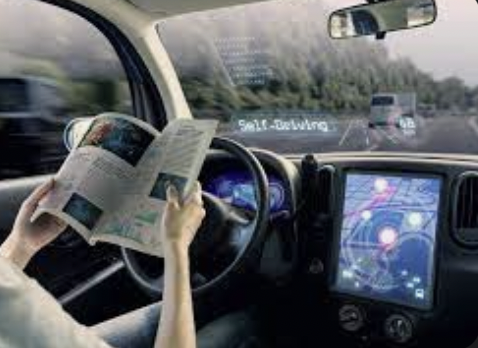
\includegraphics[width=5cm, height=4cm]{selfdriving cars}}
\caption{Self-Driving Cars}
\label{fig}
\end{figure}

\section{Conclusion}
Artificial intelligence (AI) is intelligence—perceiving, synthesizing, and inferring information—demonstrated by machines, as opposed to intelligence displayed by non-human animals and humans. Example tasks in which this is done include speech recognition, computer vision, translation between (natural) languages, as well as other mappings of inputs.\\


\section*{Acknowledgment}
Thank you for giving me this opportunity to learn this topic \LaTeX. I would also like to thank my faculty of DTL who always answered all our queries and helped us for better understanding of the subject.


\begin{thebibliography}{100} 
\bibitem{}https://idhjournal.com/article/S2468-0451(18)30144-5/fulltext
\bibitem{} https://towardsdatascience.com/advantages-and-disadvantages-of-artificial-intelligence-182a5ef6588c
\bibitem{} Kehua Su, Jie Li and Hongbo Fu, \emph{“AI and Innovation."},vol.  136, 1098-1107. 
\bibitem{Pan} Schnitzenbaumer KJ, Dukovic G. (2014). Chalcogenide-Ligand  Passivated  CdTe  Quantum  Dots  Can  Be Treated  as  Core/Cities in India.  \emph{The Journal  of Developments in AI}, Vol.2, C, 118(48): 28170-28178. 
\end{thebibliography}


\end{document}